\subsection{Direct local-field contact: protocol, readout, and limitations}
\label{sec:direct_contact_protocol}
The task is to regulate horizontal position $x$ and the vertical force
component $\lambda$ through a material/actuator change. The learner adapts all
$24$ entries of a local $3\times8$ field; its learned relations determine the
input-rate commands. This direct-field study is distinct from the retained
coefficient-family reconstruction and its geometry-dependent normal-force task.

\paragraph{Physical relation and observations}
The simulator uses $\dot p=Bu$, $p=(x,y)^{\mathsf T}$, and
\begin{align}
 \dot\lambda&=a\{h(x)-y\}-4\lambda+b\{h'(x)\dot x-\dot y\},\nonumber\\
 h(x)&=.035\sin2x+.020\cos5x.
 \label{eq:direct_contact_plant}
\end{align}
Initially $(a,b)=(600,240)$ and
$B=\left[\begin{smallmatrix}1&.15\\-.08&.85\end{smallmatrix}\right]$.
At $60$ s they change to $(1000,360)$ and
$B=\left[\begin{smallmatrix}.8&.22\\-.12&.65\end{smallmatrix}\right]$
without informing the learner. The initial state is
$(x,y,\lambda)=(0,.020-4/150,4)$.
The observed context and fixed units are
\begin{align}
 z&=(x,y,\lambda,v_x,v_y,r,u_1,u_2),\quad r=\dot\lambda,\nonumber\\
 D&=\operatorname{diag}(.3,.03,5,.15,.03,5,.15,.03),\quad
 v=D^{-1}\dot z.\label{eq:direct_contact_units}
\end{align}
On each smooth material branch, the plant obeys the three implicit relations
\begin{equation}
 f(z)=\begin{bmatrix}
 r-a\{h(x)-y\}+4\lambda-b\{h'(x)v_x-v_y\}\\
 v_x-B_{11}u_1-B_{12}u_2\\
 v_y-B_{21}u_1-B_{22}u_2
 \end{bmatrix}=0.
 \label{eq:direct_contact_relation}
\end{equation}
Writing $\gamma=a h'(x)+b h''(x)v_x$, the true field $F=D_zf$ is
\begin{equation}
 F=\begin{bmatrix}
 -\gamma&a&4&-b h'(x)&b&1&0&0\\
 0&0&0&1&0&0&-B_{11}&-B_{12}\\
 0&0&0&0&1&0&-B_{21}&-B_{22}
 \end{bmatrix}.
 \label{eq:direct_contact_true_field}
\end{equation}
Thus $F\dot z=0$ relates motion, force variation and actuation. These formulas
are simulator/evaluator-only: neither $f,F$ nor $a,b,B,h$ enters the learner or
controller. Supplied choices are context, units, three-constraint dimension,
initialization, learning settings and task references. A noise-free ideal
sensor supplies $z$ and its physical rate, including force rate and force
acceleration, from forward physics; no differentiation of noisy force data
is tested.

Commands are piecewise linear. At a sample, the observed rate is the left-hand
rate produced by the preceding command slope; the newly computed slope acts
over the next interval. At the material/actuator change, the sensor reports
the new branch's finite one-sided rates. The jump impulse of a discontinuous
context component is not assimilated as an ordinary derivative sample.
This is a piecewise-smooth simulation, not an impact or impulse-observation
model. The state is advanced by RK4 with the interval's appropriate material
branch and linearly varying command.

\paragraph{Direct learning from measured rates}
For seed $s$, a QR factorization of a generic $8\times3$ Gaussian matrix with
RNG seed $s+10000$ gives $Q_0$; $R_0=0$. The learned physical field is
$\widehat F=QD^{-1}$, with incompatibility $Qv=\widehat F\dot z$.
No entry is fixed to zero, one, or a prescribed sign, and no sparsity or
coefficient ties are imposed. The rows are normalized by the executed law:
\begin{align}
 \dot R&=vv^{\mathsf T}-.5R,\qquad QQ^{\mathsf T}=I_3,\nonumber\\
 \dot Q&=-100\{QR-(QRQ^{\mathsf T})Q\}.
 \label{eq:direct_contact_law}
\end{align}
At each $0.01$-s sample, the pre-update $Q$ forms the command and scores the
observed incompatibility. The current observed $v$ is then held during the
learning interval. Its covariance is integrated exactly as
$R(s)=e^{-.5s}R_n+2(1-e^{-.5s})v_nv_n^{\mathsf T}$, and DOP853 integrates
$Q$ against this evolving covariance, with relative/absolute tolerances
$10^{-10}/10^{-12}$. An endpoint polar correction removes numerical drift;
a raw orthogonality error greater than $10^{-7}$ aborts the run. An
instantaneous eigensolver is not substituted for the learning dynamics.
The evaluator obtains physical partials only after command construction.
Learning remains active for all $120$ s; at $40$ s, open-loop probing gives
way to feedback control.

\paragraph{Comparing learned and true partial relations}
Row-space agreement is measured in the fixed units by
$e_P=\|Q^{\mathsf T}Q-T^{\mathsf T}T\|_F$, where
$T=\{(FD)(FD)^{\mathsf T}\}^{-1/2}FD$ is the orthonormal true row frame.
For entrywise comparison, if $TQ^{\mathsf T}=U\Sigma V^{\mathsf T}$,
compare $OQ$ with $T$, where $O=UV^{\mathsf T}$ is evaluator-only.
This orthogonal alignment preserves column norms and row-space geometry,
not individual entry amplitudes. It does not enter learning or control;
the comparison concerns normalized partial relations, not unique canonical
values of $F$. For seed $101$ during control,
$\min\sigma(TQ^{\mathsf T})=.940553$; the orthogonal-factor error is below
$3.1\,10^{-15}$. The actual learned control block has minimum singular value
$.054216$, compared with $.127422$ for the orthonormal physical control block.
Small incompatibility is not reported as exact physical identification.

Canonical normalization fixes the $(r,u_1,u_2)$ columns $(6,7,8)$ by
inverting their unscaled learned block, whose minimum singular value reaches
$6.06\,10^{-6}$. This poorly conditioned inversion can produce inaccurate
material entries (Fig.~\ref{fig:direct_contact_canonical}). The controller
instead supplies $\dot r$ and solves the scaled $(v_y,u_1,u_2)$ block
$(5,7,8)$ for $(\dot v_y,\dot u_1,\dot u_2)$. Its regular completion can
therefore support useful regulation while the different canonical inversion
amplifies field errors. The evidence supports approximate local row-space
tracking, not precise material magnitudes, global integrability, or
unrestricted plant identification.
For seed $101$ in the primary window, the empirical bottom-three memory
subspace has mean projector distance $.28834$ from the physical row space,
while the learner--memory distance is $.09478$ and the third/fourth eigengap
is $.0003995$. These distinct diagnostics expose local-history bias and
tracking lag, rather than interpreting covariance positivity as physical
persistent excitation.

\begin{figure*}[p]
\centering
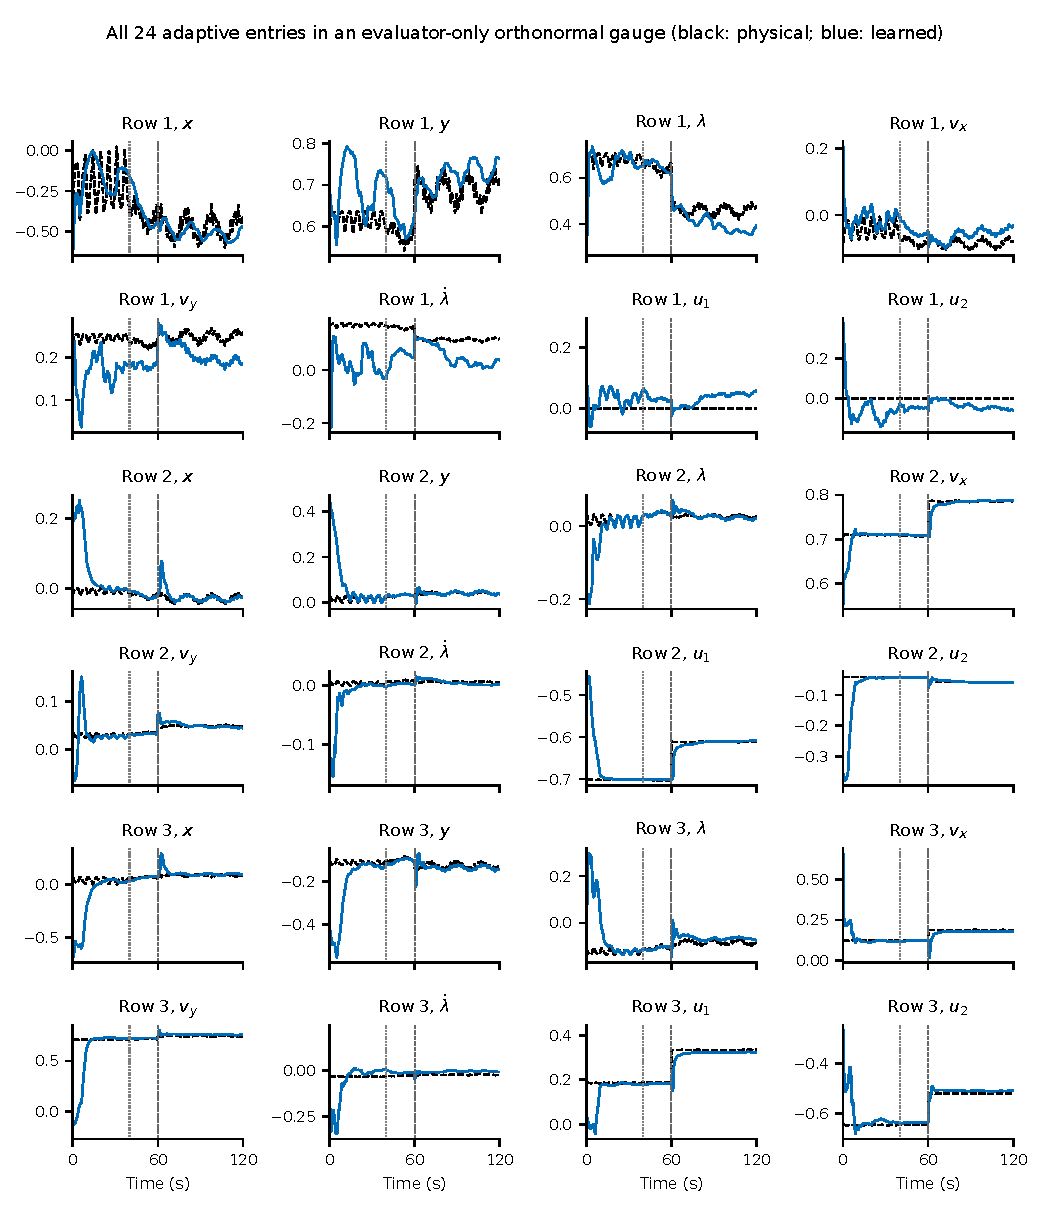
\includegraphics[width=\textwidth]{figures/direct_contact_all24.pdf}
\caption{Learning the contact relation: all $24$ adaptive entries for
preselected seed $101$. Each panel compares the same entry of the normalized
true field $T$ (black dashed) and aligned estimate $OQ$ (blue), using the
fixed units and evaluator-only orthogonal alignment defined in the text.
The learner receives no entries of $F$. Open-loop probing ends and control
begins at $40$ s (dotted line); learning continues throughout all $120$ s.
The material/actuator change occurs at $60$ s (dashed line).
Residual discrepancies remain visible; task success is not exact recovery
of every physical partial.}
\label{fig:direct_contact_all24}
\end{figure*}
\begin{figure}[t]
\centering
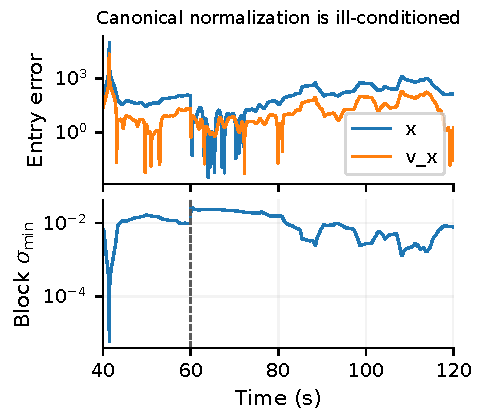
\includegraphics[width=\columnwidth]{figures/direct_contact_canonical_gauge_limitation.pdf}
\caption{A retained limitation: normalizing the material force-rate entry to
one is poorly conditioned and yields large physical-entry errors. This
normalization is evaluator-only and never used for commands or learning.}
\label{fig:direct_contact_canonical}
\end{figure}

\paragraph{Feedback and learned-field readout}
A measured open-loop warmup occupies $0\le t<40$ s:
\begin{align}
 u_1(t)&=.06\sin1.1t+.03\sin(2.3t+.4)\nonumber\\
       &\quad+.015\sin(3.7t+.2),\nonumber\\
 u_2(t)&=.002\sin(.9t+.8)+.0015\sin1.9t\nonumber\\
       &\quad+.001\sin(3.1t+.1).
 \label{eq:direct_contact_probe}
\end{align}
The applied warmup slope is the forward difference of these prescribed input
values across the next sample interval. This is an ordinary observed temporal
trajectory, not a source of independently labeled perturbation tangents.
After warmup, with $s=t-40$, the references are
\begin{align}
 x_d&=.03\sin(.35s)+.01\sin(2.3s)+.005\sin(3.7s),\nonumber\\
 \lambda_d&=4+.2\sin(.5s)+.08\sin(1.9s)+.04\sin(3.1s).
 \label{eq:direct_contact_reference}
\end{align}
Their derivatives are known task inputs; small independent components maintain
local excitation. Feedback prescribes $\dot v_x=a_x^*$ and
$\dot r=a_\lambda^*$:
\begin{align}
 a_x^*&=\ddot x_d-4(v_x-\dot x_d)-4(x-x_d),\nonumber\\
 a_\lambda^*&=\ddot\lambda_d-6(\dot\lambda-\dot\lambda_d)
                         -9(\lambda-\lambda_d).
 \label{eq:direct_contact_feedback}
\end{align}
The supplied rates are $(v_x,v_y,r,a_x^*,a_\lambda^*)$; the computed
rates are $(a_y,\dot u_1,\dot u_2)$. Using one-based columns
$S=(1,2,3,4,6)$ and $C=(5,7,8)$, the same pre-update relation
$\widehat F\dot z=0$ gives
\begin{equation}
 \begin{bmatrix}a_y\\\dot u_1\\\dot u_2\end{bmatrix}
 =-D_CQ_C^{-1}Q_SD_S^{-1}
 \begin{bmatrix}v_x\\v_y\\r\\a_x^*\\a_\lambda^*\end{bmatrix}.
 \label{eq:direct_contact_completion}
\end{equation}
Desired rates enter this query only; learning still uses observed $v$.
Only the last two completed components are applied: their limited slopes
update the measured input by $u_{n+1}=u_n+\Delta t\,\dot u_n$.
The inferred $a_y$ closes the relation but is not a separate actuator command.
Limits are $|u_i|\le.8$ and $|\dot u_i|\le5$.
If $\sigma_{\min}(Q_C)<.005$, the trajectory is recorded as failed and stops;
there is no physical inverse or fallback controller. Domain checks stop a run
if indentation or force is nonpositive, $|x|>1$, $|y|>.3$, or $|\lambda|>100$.
The prescribed control law contains neither $a,b,B$ nor $h$.

\paragraph{Task results and retained failures}
Exploratory seed $0$ was separate from confirmation. Its first, less excited
reference reached a readout guard at $58.58$ s and is retained as a failure.
The local references in~(\ref{eq:direct_contact_reference}) completed both a
60-s constant-plant pilot and a 120-s pilot with the scheduled change.
The learning gain, memory, units, and guard were unchanged. The measured
conditioning and task response motivated the reference revision; physical
partial errors were not feedback or selection inputs.

The complete protocol and source hashes were fixed before seeds
$101$--$105$, with seed $101$ preselected for illustrations. These seeds vary
generic field initialization; they are not five independently drawn plants or
noise realizations. The declared primary window was $[110,120)$ s. Criteria
required complete 120-s trajectories, no domain/guard/saturation event,
position RMSE below $.01$, vertical-force RMSE below $.2$, mean row-projector
error below $.6$, and field, incompatibility, and query errors below half their
respective frozen-initial same-stream values. All five runs met these
criteria; no seed was discarded.

\begin{table}[t]
\centering\small\setlength{\tabcolsep}{2.5pt}
\caption{All declared direct-contact runs, primary window $[110,120)$ s.
$e_P=\|Q^{\mathsf T}Q-P_{FD}\|_F$ in the fixed units of
(\ref{eq:direct_contact_units}). Query error is RMS norm over all three
completed physical rates. The frozen estimate is a same-stream shadow.}
\label{tab:direct_contact_seeds}
\begin{tabular}{rccccc}
\hline
Seed & Force RMSE & Position RMSE & Mean $e_P$ & Query RMS & Pass\\
\hline
101 & .121637 & $6.8111\,10^{-5}$ & .298169 & .00717262 & Yes\\
102 & .121637 & $6.8110\,10^{-5}$ & .298169 & .00717265 & Yes\\
103 & .121636 & $6.8112\,10^{-5}$ & .298169 & .00717260 & Yes\\
104 & .121642 & $6.8105\,10^{-5}$ & .298170 & .00717283 & Yes\\
105 & .121636 & $6.8113\,10^{-5}$ & .298169 & .00717260 & Yes\\
\hline
\end{tabular}
\end{table}
Across the five seeds, force RMSE is $.121638\pm2.31\,10^{-6}$,
position RMSE is $(6.81102\pm.00031)10^{-5}$, and mean projector error is
$.298169\pm6.15\,10^{-7}$ (sample standard deviations). The frozen projector
error is $1.93389\pm.16981$. Mean incompatibility norm is $.00359588$ versus
$.511730$ for frozen initialization. Query RMS is $.00717266\pm9.66\,10^{-8}$
versus $.214812\pm.100090$ for the frozen shadow. Query comparison supplies
the same requested rates to the learned and physical fields; it is an
inverse-readout diagnostic, not an independent future-prediction experiment.
Own-trajectory force/motion errors separately test the applied readout.

\paragraph{Numerical and provenance checks}
Saved records include every pre-update $Q,R,z,\dot z$, command, supplied query,
physical evaluator field, source snapshot, configuration, and per-file hash.
Recalculation from raw records reproduced trace metrics and controller outputs.
The covariance transition error is at most $1.12\,10^{-14}$; independent
200-substep RK4 checks of selected learning intervals agree within
$2.57\,10^{-12}$ in $Q$. Every entry changed, with the smallest across-entry
maximum change exceeding $.1185$ over the audited runs. Directional finite
differences check the evaluator partials separately from the learning rule.

The predeclared seed-$101$ refinement halves the observation/plant step to
$.005$ s, with all other settings unchanged. It also completes and passes the
criteria. Its force RMSE is $.109237$, versus $.121637$ at $.01$ s; projector
error is $.297450$, versus $.298169$. The same-time late force trajectories
differ by RMS $.01490$ N, and projector-error traces by RMS $.001719$.
Thus qualitative success is preserved, but fine quantitative force accuracy
is discretization-sensitive; the coarse records have not been replaced or
called a converged continuous-time solution.

The portable implementation, frozen protocol, auditing and plotting programs
are under \texttt{experiments/direct\_submission/contact/}. This new identity
has nine recorded executions: three exploratory cases, five confirmation
seeds, and one refinement. The earlier experiments using noisy measured
signals and cascaded causal differentiation are different protocols; their
failures remain archived and do not establish robustness for this study.
Local records and hashes are evidence of execution,
not a claim that a new archive or code revision has already been published.
